\documentclass[twoside,a4paper,11pt,addpoints,answers]{exam}%answers,answers,


\title{XX 1}
\date{}
\author{Juliette Fenogli}


\usepackage{siunitx}
\usepackage{mystyles}
\usepackage[export]{adjustbox}
\usepackage{mathpazo}
\usepackage{booktabs}
\usepackage{framed}
\usepackage{mdframed}
\usepackage[most]{tcolorbox}
\usepackage{listings}
\usepackage{mhchem}
\usepackage{tcolorbox}

\usepackage{subfig}
\usepackage{float}

\usepackage{adjustbox}

\lstset
{upquote=true,
columns=flexible,
    basicstyle=\small\tt\hbox{}, 
	basicstyle=\ttfamily,
	language=Python,
    framesep=\fboxsep,
    framerule=\fboxrule,
    xleftmargin=\dimexpr\fboxsep+\fboxrule,
    xrightmargin=\dimexpr\fboxsep+\fboxrule,
	commentstyle=\color{gray},
	frame=single,
	rulecolor=\color{green!5},
	backgroundcolor=\color{gray!5},
	breaklines,
	numbers=left, 
	numbersep=5pt,  
	numberstyle=\scriptsize \ttfamily\color{gray},
	breakindent=1.5em,
	literate={Δ}{{$\mathtt{\Delta}$}}1 {‡}{{$\mathtt{\ddagger}$}}1
  {á}{{\'a}}1 {é}{{\'e}}1 {í}{{\'i}}1 {ó}{{\'o}}1 {ú}{{\'u}}1
  {Á}{{\'A}}1 {É}{{\'E}}1 {Í}{{\'I}}1 {Ó}{{\'O}}1 {Ú}{{\'U}}1
  {à}{{\`a~}}1 {è}{{\`e}}1 {ì}{{\`i}}1 {ò}{{\`o}}1 {ù}{{\`u}}1
  {À}{{\`A~}}1 {È}{{\'E}}1 {Ì}{{\`I}}1 {Ò}{{\`O}}1 {Ù}{{\`U}}1
  {ä}{{\"a}}1 {ë}{{\"e}}1 {ï}{{\"i}}1 {ö}{{\"o}}1 {ü}{{\"u}}1
  {Ä}{{\"A}}1 {Ë}{{\"E}}1 {Ï}{{\"I}}1 {Ö}{{\"O}}1 {Ü}{{\"U}}1
  {â}{{\^a}}1 {ê}{{\^e}}1 {î}{{\^i}}1 {ô}{{\^o}}1 {û}{{\^u}}1
  {Â}{{\^A}}1 {Ê}{{\^E}}1 {Î}{{\^I}}1 {Ô}{{\^O}}1 {Û}{{\^U}}1
  {œ}{{\oe}}1 {Œ}{{\OE}}1 {æ}{{\ae}}1 {Æ}{{\AE}}1 {ß}{{\ss}}1
  {ç}{{\c c}}1 {Ç}{{\c C}}1 {ø}{{\o}}1 {å}{{\r a}}1 {Å}{{\r A}}1
  {€}{{\EUR}}1 {£}{{\pounds}}1 {×}{{$\times$}}1,       
}


\usepackage{adjustbox}
\usepackage{colortbl}
\usepackage{fontawesome}
\usepackage{todonotes}
\usepackage{listings} %codes python
\usepackage{parskip}

%Columns Spacing
\newcolumntype{C}[1]{>{\centering\let\newline\\\arraybackslash\hspace{0pt}}m{#1}}
\newcolumntype{M}[1]{>{\centering\arraybackslash}m{#1}}

%Colorbox
\newtcolorbox{mybox}{colback=white!5!white,
colframe=black!75!black,left=7mm}

\newcounter{foo} %Counter questions

\begin{document}

\begin{minipage}{0.33\textwidth}
Noms-Prénoms du binôme
\end{minipage}\begin{minipage}{0.33\textwidth}
$n^\circ 1$ :
\end{minipage}\begin{minipage}{0.33\textwidth}
$n^\circ 2$ :
\end{minipage}



\tito{Synthèse et caractérisation d'un matériau d'électrode $\oplus$ pour un accumulateur lithium-ion}

\paragraph*{But} 

Bienvenue à IUTEnergy, une compagnie qui conçoit et assemble des solutions de stockage d'énergie électrochimique. Suite à votre recrutement, la feuille de route de la Fig. \ref{fig:01} est proposée afin d'évaluer vos compétences de techniciens matériaux.

\begin{center}
\begin{minipage}{0.58\textwidth}

\includegraphics[width=\textwidth]{figures/Fig01}
\end{minipage}\hfill\begin{minipage}{0.38\textwidth}
\captionof{figure}{Bloc diagramme des différentes étapes de la synthèse et de la caractérisation d'un dioxyde de manganèse lithié \ce{LiMn2O4}}
\label{fig:01}
\end{minipage}
\end{center}

Tout l'enjeu de cette entrevue est de montrer votre capacité à justifier le protocole proposé et à élaborer un oxyde métallique. Ce sera utilisé par la suite dans la conception d'un accumulateur lithium-ion, sous forme de bouton.



\paragraph*{Quelques remarques :}
\begin{enumerate}
\item La lecture des annexes du TP doit être fait en amont.
\item Toute figure doit comporter des axes, des unités, un titre et des légendes. Le titre doit permettre à l'enseignant de comprendre l'essentiel de la figure sans avoir à lire le texte associé.
\item Toute donnée expérimentale doit être accompagnée des conditions expérimentales et d'une indication sur les outils de mesure utilisés.
\item Les questions en {\color{purple} violet} doivent avoir été réfléchies en amont du TP. En l'absence de recherche de votre part, l'enseignant en charge du TP sanctionnera le binôme.
\end{enumerate}

\faWarning ~ Il est impératif de prévoir une feuille de route avec son binôme afin que les caractérisations soient conduites simultanément aux étapes de synthèse. La répartition du travail expérimental au sein du binôme doit permettre de faire entrer le TP dans les \SI{4}{\hour} dédiées.

\tableofcontents

\section{Synthèse du précurseur \ce{MnCO3} [Synthèse - \faClockO ~ \SI{1}{\hour} - Caractérisation - \faClockO ~ \SI{30}{\minute}]}

\paragraph*{Protocole}

\begin{enumerate}
\item Dissoudre $m_1$ \si{\gram} de \ce{MnSO4 (s)} dans \SI{40}{\milli\liter} d'eau distillée.
\item Mettre sous agitation la solution de \ce{MnSO4 (aq)} et la chauffer à \SI{60}{\celsius}. 
\item Dissoudre $m_2$ \si{\gram}  \ce{Na2CO3 (s)} dans \SI{20}{\milli\liter} d'eau distillée. 
\item la solution de \ce{Na2CO3 (aq)} est ensuite ajoutée doucement, sous agitation et à la burette, à la solution de \ce{MnSO4 (aq)}. Une fois la burette vide, on patiente \SI{10}{\minute}, sous agitation, puis on filtre le précipité sur un entonnoir de Büchner et on sèche le précipité à l'étuve à \SI{90}{\celsius} pendant \SI{30}{\minute} sur un verre de montre.
%en ayant les mêmes quantités de matière pour les deux réactifs. 
\item Mesurer la masse du produit de synthèse.
\end{enumerate}

\faWarning ~ Attention à conserver de l'échantillon avant et après calcination pour les analyses à faire.

\paragraph*{Données expérimentales à annoter}

\begin{center}
\begin{tabular}{|c|c|c|c|c|}
\hline
 & \ce{Na2CO3 (s)} & \ce{MnSO4.H2O (s)} & Verre de montre & Verre de montre + produit de synthèse \\
\hline
Masses & & &  & \\
\hline
\end{tabular}
\end{center}

\paragraph*{Questions}

On admettra que \ce{MnSO4 (s)} et \ce{Na2CO3 (s)} se dissocient quantitativement dans l'eau à \SI{60}{\celsius}.

\begin{questions}
\question[1\half] \label{Q:1-01} {\color{purple} Donner les equations de dissociations des sels \ce{MnSO4} et \ce{Na2CO3} dans l'eau distillée. En déduire l'équation de réactions associée à la formation de \ce{MnCO3 (s)}. De quel type de réaction s'agit-il ?}

\begin{mybox}
\begin{solution}[4cm]
\underline{\'{E}quations de dissociations}
\begin{align*}
\ce{MnSO4 (s) &= Mn^{2+} (aq) + SO4^{2-} (aq)} \\
\ce{Na2CO3 (s) &= 2 Na^+ (aq) + CO3^{2-} (aq)}
\end{align*}
\underline{\'{E}quation de précipitation}
\begin{align*}
\ce{Mn^{2+} (aq) + CO3^{2-} (aq) = MnCO3 (s)}
\end{align*}
\end{solution}
\end{mybox}


On va chercher à synthétiser environ \SI{1.8}{\gram} d'oxydes de manganèse lithié \ce{LiMn2O4}. Il a été estimé qu'il faudrait environ \SI{2.3}{\gram} de carbonate de manganèse \ce{MnCO3} pour y parvenir.

\question[1\half] {\color{purple} Calculer les masses $m_1$ et $m_2$ en utilisant des conditions st{\oe}chiométriques.}

\begin{mybox}\begin{solution}[6cm]
Les étudiants vont synthétiser \SI{1.8}{\gram} d'oxyde de manganèse lithié \ce{LiMn2O4}, dont \SI{0.3}{\gram} servira dans la réalisation de chaque cathode.
En s'appuyant sur la réponse à la Q. \ref{Q:1-01}, on peut écrire l'égalité suivante : 
\begin{align*}
n_0 (\ce{CO3^{2-}}) &= n_0 (\ce{Mn^{2+}}) = n_\infty ( \ce{MnCO3} ) \\
n_0 (\ce{Na2CO3}) &= n_0 (\ce{MnSO4}) = n_\infty ( \ce{MnCO3} ) \\
\frac{m_0 (\ce{Na2CO3})}{M (\ce{Na2CO3})} &= \frac{m_0 (\ce{MnSO4.H2O})}{M (\ce{MnSO4.H2O})} = \frac{m_\infty ( \ce{MnCO3} )}{M( \ce{MnCO3} )}
\end{align*}

%Na2CO3 : 497-19-8, MnSO4.H2O 10034-96-5 (demander à Chabane de vérifier)
%Li2CO3 554-13-2
On trouve deux relations :
\begin{align*}
m_0 (\ce{Na2CO3}) & = \frac{M (\ce{Na2CO3})}{M( \ce{MnCO3} )} m_\infty ( \ce{MnCO3} ) \\
m_0 (\ce{MnSO4.H2O}) & = \frac{M (\ce{MnSO4.H2O})}{M( \ce{MnCO3} )} m_\infty ( \ce{MnCO3} )
\end{align*}

%105.99 g/mol Na2CO3, MnSO4.H2O 169.02 g/mol, MnCO3 114,9469 g/mol
\underline{Application Numérique} (2 CS)
\begin{align*}
m_0 (\ce{Na2CO3}) &= 2.1 ~ \si{\gram}\\
m_0 (\ce{MnSO4.H2O}) &= 3.4 ~ \si{\gram}
\end{align*}
\end{solution}\end{mybox}

Il a été observé expérimentalement qu'une augmentation de la concentration de carbonate diminue la proportion de \ce{Mn} dans le filtrat (obtenu après une filtration sur Büchner).

\question[1] {\color{purple} En vous appuyant sur la loi d'action des masses (loi de Guldberg \& Waage), montrer que la thermodynamique prédit cette évolution.}

\begin{mybox}\begin{solution}[3cm]
\`{A} l'équilibre thermodynamique et en se plaçant dans l'idéalité, on a :
\begin{align*}
K_s ( \ce{MnCO3} ) = \frac{[\ce{Mn^{2+}}][\ce{CO3^{2-}}]}{c^{\circ 2}}
\end{align*}
En différenciant, on a :
\begin{align*}
d [ \ce{Mn^{2+}} ] = - \frac{[\ce{Mn^{2+}}]}{[\ce{CO3^{2-}}]} d [\ce{CO3^{2-}}]
\end{align*}

Or, si on a : $[\ce{CO3^{2-}}] ~ \nearrow \implies d[\ce{CO3^{2-}}] > 0 \implies d[\ce{Mn^{2+}}] < 0 \implies [\ce{Mn^{2+}}] ~ \searrow$

L'augmentation de la concentration de carbonate améliore la proportion de manganèse précipité.
\end{solution}\end{mybox}

Les données thermodynamiques suivantes sont établies à \SI{298}{\kelvin} : 

\begin{center}
\begin{minipage}{0.48\textwidth}
\begin{tabular}{cc}
\toprule
Constituant & Enthalpie de formation standard \\
& \si{\kilo\joule\per\mole} \\
\midrule
%\ce{CO3^{2-} (aq)} & -677.14 \\
\ce{Na^+ (aq)} & -240.12 \\
\ce{Mn^{2+} (aq)} & -220.8 \\
\ce{Na2CO3 (s)} & -1130.77 \\
\ce{MnCO3 (s)} & -881.7 \\
\bottomrule
\end{tabular}
\end{minipage}\begin{minipage}{0.48\textwidth}
\captionof{figure}{Enthalpies de formations de quelques solides et espèces en solution aqueuses à \SI{298}{\kelvin}}
\end{minipage}
\end{center}

\hspace{0.5cm}

Les chercheurs ont établi que l'énergie d'activation de la réaction de formation du carbonate de manganèse à partir du sulfate de manganèse vaut \SI{27.19}{\kilo\joule\per\mole}.

Le protocole encourage à réaliser la synthèse du solide à \SI{60}{\celsius}.

\question[1] {\color{purple} Définir l'énergie d'activation. Dans quelle loi cette grandeur rentre en jeu ? Vous définirez les termes de cette loi et vous en donnerez les unités. En déduire l'influence de la température sur la vitesse de réaction.}

\begin{mybox}\begin{solution}[3cm]
L'énergie d'activation est la différence d'énergie entre l'état réactif et l'état de transition et est notée $E_A$ ou $E^\pm$. Elle intervient dans la loi d'Arrhenius, qui s'exprime comme : 
\begin{align*}
k(T) = A \exp \left( - \frac{E_A}{RT} \right)
\end{align*}

où $A$ est le pré-facteur exponentiel [$\si{\mole^{1-n}\liter^{-1+n}\second^{-1}}$], $E_A$ l'énergie d'activation [\si{\joule\per\mole}], $R$ la constante des gaz parfait [\si{\joule\per\mole\per\kelvin}] et $T$ la température [\si{\kelvin}].

La loi d'Arrhenius montre bien que $T ~ \nearrow \implies k(T) ~ \nearrow \implies v ~ \nearrow$.

\end{solution}\end{mybox}%WARNING

\question[1] {\color{purple} \`{A} partir des données thermodynamiques, évaluer l'enthalpie de réaction associée à la réaction de formation du carbonate de manganèse à partir du carbonate de sodium. Commenter l'influence de la température, d'un côté, sur le déplacement d'équilibre et d'un autre côté, sur la vitesse de réaction. Identifier le compromis que les chimistes des matériaux ont dû trouver lors de cette synthèse.}

\begin{mybox}\begin{solution}[3cm]
\underline{Equation de réaction :}
\begin{align*}
\ce{Na2CO3 (s) + Mn^{2+} (aq) = MnCO3 (s) + 2 Na^+ (aq)}
\end{align*} 

\underline{Calcul de l'enthalpie de réaction}
\begin{align*}
\Delta_r H^\circ &= 2 \Delta_f H^\circ ( \ce{Na^{+} (aq)} ) + \Delta_f H^\circ ( \ce{MnCO3} ) - \Delta_f H^\circ ( \ce{Mn^{2+} (aq)} ) - \Delta_f H^\circ ( \ce{Na2CO3 (s)} ) \\
&\stackrel{AN}{=} -10.37 ~ \si{\kilo\joule\per\mole}
\end{align*}
La réaction est exothermique (loi de van't Hoff), donc lorsque $T ~ \nearrow \implies \text{favorisé dans le sens indirect} \ce{<-}$.
\end{solution}\end{mybox}

\question[2] Réaliser l'acquisition du diffractogramme sur poudre de votre produit de synthèse. Identifier la (ou les) phase(s) formée(s).

\begin{mybox}\begin{solution}[6cm]

\begin{center}
\begin{minipage}{0.68\textwidth}

\includegraphics[width=\textwidth]{figures/Corr01}
\end{minipage}\begin{minipage}{0.28\textwidth}
\captionof{figure}{Diffractogramme sur poudre du carbonate de manganèse \ce{MnCO3} comparé à une référence pour $\lambda = 1.542 ~ \si{\angstrom}$.}
[marque : Aeris Malvern PANalytical, $2\theta_{min} = 10.001 ~ \si{\degree}$, $2\theta_{max} = 70 ~ \si{\degree}$, $2 \Delta \theta = 0.0027166 ~ \si{\degree}$, durée d'acquisition : $59.925 ~ \si{\second\per{mesure}}$]
\end{minipage}
\end{center} %WARNING

\underline{Observations} Bonne corrélation des pics, unique phase formée est bien \ce{MnCO3 (s)} cristallisé.

\faWarning ~ L'échantillon réalisé à l'IUT présente un décalage systématique car la surface de la poudre n'était pas plane.
\end{solution}\end{mybox}
%WARNING
Dans les travaux de Ali \& al. (doi : 10.1080/00986445.2020.1839434), les signaux infrarouges suivants ont été observés et affectés : 
\begin{center}
\begin{minipage}{0.68\textwidth}
\begin{tabular}{cccc}
\toprule
Nombre d'onde & Intensité & Largeur & Affectation \\
\si{\per\centi\meter} & & & \\
\midrule
613 & moyenne & fine & \ce{CO3^{2-}}, flexion \ce{O-C-O} \\
714 & moyenne & fine & \ce{CO3^{2-}}, flexion \ce{C-O} \\
866 & forte & fine & \ce{CO3^{2-}}, flexion \ce{O-C-O} \\
1083 & forte & large & \ce{CO3^{2-}}, élongation \ce{C-O} \\
1400 & forte & large &  \ce{CO3^{2-}}, élongation \ce{C-O} \\
1638 & faible & moyenne & \ce{H2O}, flexion \ce{O-H} \\
3281 & faible & large & \ce{H2O}, élongation \ce{O-H} \\
\bottomrule
\end{tabular}
\end{minipage}\begin{minipage}{0.28\textwidth}
\captionof{table}{Table des bandes infrarouges associées au produit de synthèse de Ali \& al.}
\end{minipage}
\end{center}


\question[1\half] Réaliser l'acquisition du spectre infrarouge de votre produit de synthèse, identifier les bandes d'absorption et vérifier la présence d'ions carbonates et d’éventuelles molécules d'eau. 
\begin{mybox}\begin{solution}[6cm]
\begin{center}
\begin{minipage}{0.68\textwidth}

\includegraphics[width=\textwidth]{figures/Corr02}
\end{minipage}\begin{minipage}{0.28\textwidth}
\captionof{figure}{Spectre infrarouge du carbonate de manganèse \ce{MnCO3} après séchage}
[$\bar{\nu}_{min} = 450 ~ \si{\per\centi\meter}$, $\bar{\nu}_{max} = 4000 ~ \si{\per\centi\meter}$, superposition de 4 scans]
\end{minipage}
\end{center}
\underline{Observations}
\begin{itemize}
\item présence d'ions carbonates,
\item absence de molécules d'eau.
\end{itemize}
\end{solution}\end{mybox}

\question[1] Après avoir validé ou invalidé la pureté du produit de synthèse, calculer le rendement de cette première étape.

\begin{mybox}\begin{solution}[4cm]

Si l'échantillon est pur et composé d'une unique phase \ce{MnCO3} (cf l'ensemble des analyses réalisées précédemment). 

\begin{align*}
n_0 ( \ce{MnSO4.H2O} ) &= \frac{m_{reactif} (\ce{MnSO4.H2O} )}{M ( \ce{MnSO4} )} \\
n_\infty ( \ce{MnCO3} ) &= \frac{m_{produit}}{ M (\ce{MnCO3}) }
\end{align*}
On trouve au final un rendement :
\begin{align*}
r_1 = \frac{n_\infty ( \ce{MnCO3} )}{n_0  ( \ce{MnSO4.H2O} )}
\end{align*}
\underline{AN}
\faWarning ~ Les étudiants pouvaient trouver parfois des rendement supérieures à \SI{100}{\percent} qui traduisent un séchage partiel de leurs poudres initiales. Dans ce cas, deux possibilités : les étudiants sont suffisamment bien avancés pour laisser une dizaine de minutes de plus leur échantillon à l'étuve ; les étudiants sont en retard, auquel cas ils commentent la valeur aberrante obtenue.
\end{solution}\end{mybox}

\setcounter{foo}{\value{question}}
\end{questions}

\paragraph*{Données :}
\begin{itemize}
\item Masses molaires : $M( \ce{MnCO3} ) = 114.9469 ~ \si{\gram\per\mole}$
\end{itemize}

\newpage

\section{Synthèse du matériaux final \ce{LiMn2O4}  [Synthèse - \faClockO ~ \SI{1.5}{\hour} - Caractérisation - \faClockO ~ \SI{1}{\hour}]}



\paragraph*{Protocole}
\begin{itemize}
\item Réaliser un mélange homogène de \ce{LiCO3} et \ce{MnCO3} à l'aide d'un mortier ;
\item Mettre le creuset au four à \SI{790}{\celsius} pendant \SI{1}{\hour}.
\end{itemize}

\faWarning ~ Attention à conserver de l'échantillon avant et après calcination pour les analyses à faire.

\paragraph*{Données expérimentales à annoter}
\begin{center}
\begin{tabular}{|c|c|c|c|}
\hline
 & \ce{Li2CO3 (s)} & \ce{MnCO3 (s)} & \ce{Produit final} \\
\hline
Couleurs & & & \\
\hline
\end{tabular}
\end{center}

\begin{center}
\begin{tabular}{|c|c|c|c|c|}
\hline
 & Creuset & Masse de \ce{Li2CO3 (s)} & Masse de \ce{MnCO3 (s)} & Creuset + produit final \\
\hline
Masses & & &  & \\
\hline
\end{tabular}
\end{center}

\begin{questions}
\setcounter{question}{\thefoo}

\question[1] \label{Q:2-01} {\color{purple} Calculer la masse de \ce{Li2CO3} à prélever dans le mélange pour respecter la st{\oe}chiométrie du spinelle \ce{LiMn2O4}.}

\begin{mybox}\begin{solution}[4cm]
Les précurseurs sont tels quel : 
\begin{align*}
2 n_0 ( \ce{Li2CO3 } ) &=  \frac{n_\infty ( \ce{MnCO3} )}{2} \\
m_0 ( \ce{Li2CO3} ) &=  \frac{1}{4} \frac{M ( \ce{MnCO3} )}{M ( \ce{Li2CO3} ) } m_\infty ( \ce{MnCO3} )
\end{align*}

\underline{AN}


\faWarning ~ Les étudiants doivent faire l'AN avec la masse de \ce{MnCO3} qu'ils ont obtenu à la première étape de la synthèse.

\end{solution}\end{mybox}


\question[1] \label{Q:2-02} Après avoir proposé une hypothèse simple sur la nature chimique du composé final, évaluer le rendement de cette étape de votre synthèse. Calculer le rendement de l'ensemble des deux étapes de la synthèse.

\begin{mybox}\begin{solution}[7cm]
On va supposer qu'une seule phase est formée afin d'évaluer le rendement. \\
\underline{Calcul le rendement de l'étape 2}
\begin{align*}
r_2 &= 2 \frac{n_{\infty,2} ( \ce{LiMn2O4} )}{n_{\infty,1} ( \ce{MnCO3}) } \\
&= 2 \frac{M ( \ce{MnCO3})}{M ( \ce{LiMn2O4} )} \frac{m_{\infty,2} ( \ce{LiMn2O4} )}{m_{\infty,1} ( \ce{MnCO3}) }\\
&\stackrel{AN}{=} ?
\end{align*}
\underline{Calcul du rendement des étapes 1 \& 2}
\begin{align*}
r_{tot} &= 2 \frac{n_{\infty, 2} ( \ce{LiMn2O4} ) }{n_{0} ( \ce{MnSO4 . H2O} ) } \\ 
&= \frac{n_{\infty,1} ( \ce{MnCO3})}{n_{0} ( \ce{MnSO4 . H2O} ) } \times 2 \frac{n_{\infty,2} ( \ce{LiMn2O4} )}{n_{\infty,1} ( \ce{MnCO3}) } \\
&= r_1 \times r_2 \stackrel{AN}{=} ?
\end{align*}
\faWarning ~ En cas de perte de masse lors des caractérisations (IR \& DRX), les étudiants doivent les prendre en compte si possible dans le calcul de $r_2$.
\end{solution}\end{mybox}

\question[2] \label{Q:2-03a} Caractériser, par diffraction des rayons X, la (ou les) phase(s) formée(s) suite à la synthèse.

\begin{mybox}\begin{solution}[6cm]
Les étudiants comparent leur acquisition en DRX avec la référence proposée en Sec. \ref{sec:diffracto} : \\

\begin{minipage}{0.68\textwidth}

\includegraphics[width=\textwidth]{figures/Corr03.png}
\end{minipage}\hfill\begin{minipage}{0.28\textwidth}
\captionof{figure}{Diffractogramme sur poudre du dioxyde de manganèse lithié, produit de synthèse, comparé à une référence pour $\lambda = 1.542 ~ \si{\angstrom}$.}
[marque : Aeris Malvern PANalytical, $2\theta_{min} = 10.001 ~ \si{\degree}$, $2\theta_{max} = 70 ~ \si{\degree}$, $2 \Delta \theta = 0.0027166 ~ \si{\degree}$, durée d'acquisition : $59.925 ~ \si{\second\per{mesure}}$]
\label{fig:Corr03}
\end{minipage}
\end{solution}\end{mybox}

Par cette voie de synthèse, la présence d'interférences constructives de faible intensité est souvent observée. Ces pics ont été interprétés comme la présence d'une phase non-st{\oe}chiométrique de \ce{LiMn2O4} enrichie en lithium (c.-à-d. que le ratio \ce{Li}/\ce{Mn} > 1).

\question[2] \label{Q:2-03b} En notant $1+x$ la st{\oe}chiométrie de lithium dans le spinelle, proposer un ou des motifs possibles à cette phase enrichie en lithium. Identifier les défauts ponctuels intrinsèques possibles de cette phase.

\begin{mybox}\begin{solution}[10cm]
La présence de pics non désirés est dû à la présence d'une phase enrichie en lithium, notée :
\begin{align*}
\ce{Li_{1+x} Mn_2 O4}
\end{align*}

Dans un modèle purement ionique, on observe qu'un tel écart à la st{\oe}chiométrie conduirait à l'apparition de charges positives : 
\begin{align*}
(1+x) no (Li) +  2 no ( \ce{Mn} ) + 4 no ( \ce{O} ) = x no ( \ce{Li} ) > 0
\end{align*}

Cet excès de charges positives peut-être comblé par plusieurs mécanismes possibles : 
\begin{enumerate}
\item la présence de lacunes de manganèse : 
\begin{align*}
(1+x) no (Li) +  (2-\delta) no ( \ce{Mn} ) + 4 no ( \ce{O} ) &= 0 \\
\implies x no ( \ce{Li} ) - \delta no ( \ce{Mn} ) &= 0 \\
\implies \delta &= x \frac{no ( \ce{Li} )}{no ( \ce{Mn} )}
\end{align*}

Donc le motif dans un tel mécanisme s'écrirait :
\begin{align*}
 \ce{Li_{1+x} Mn_{2 - \alpha x} O4} \text{ avec } \alpha \in [0.25, 0.33]
\end{align*}

\item l'insertion d'atomes d'oxygènes :
\begin{align*}
(1+x) no (Li) +  2 no ( \ce{Mn} ) + (4+\delta') no ( \ce{O} ) &= 0 \\
\implies x no ( \ce{Li} ) + \delta'  no ( \ce{O} ) &= 0 \\
\implies \delta' &= - x \frac{no ( \ce{Li} )}{no ( \ce{O} )}
\end{align*}

Donc le motif dans un tel mécanisme s'écrirait :
\begin{align*}
 \ce{Li_{1+x} Mn_{2} O_{4+0.5x}}
\end{align*}

\item la présence des deux mécanismes simultanément : insertion d'atomes d'oxygène + présence de lacunes de manganèse

\end{enumerate}

\faWarning ~ Accepter toute proposition de redox interne où l'étudiant propose un excès de \ce{Mn (III)} et un déficit de \ce{Mn (IV)}.

\end{solution}\end{mybox}

%\question La phase \ce{Li2Mn4O9} est un spinelle présentant des défauts. Identifier la nature éventuelle des défauts de cette phase.

\question[1\half] \label{Q:2-04} Caractériser la présence de traces d'eau ou de carbonates par spectroscopie infrarouge. Que constatez-vous ?

\begin{mybox}\begin{solution}[5cm]

On constate l'absence de bandes de vibrations d'élongation ou de flexion associées aux ions carbonates et aux molécules d'eau.

\begin{minipage}{0.68\textwidth}

\includegraphics[width=\textwidth]{figures/Corr04}
\end{minipage}\hfill\begin{minipage}{0.28\textwidth}
\captionof{figure}{Spectre infrarouge du produit final, obtenu à la fin de la seconde étape, comparé au carbonate de manganèse \ce{MnCO3} obtenu à la fin de la première étape}
[$\bar{\nu}_{min} = 450 ~ \si{\per\centi\meter}$, $\bar{\nu}_{max} = 4000 ~ \si{\per\centi\meter}$, superposition de 4 scans]
\end{minipage}
\end{solution}\end{mybox}

Afin de comprendre le comportement thermique de votre échantillon, il est possible de réaliser une analyse thermogravimétrique, dont le principe général est détaillé à la section \ref{sec:TGA}.

La séquence proposée est la suivante : 
\begin{itemize}
\item Température initiale : \SI{30}{\celsius} ;
\item Température finale : \SI{790}{\celsius} ;
\item Rampe de température : \SI{30}{\celsius\per\minute} ;%WARNING : rampe plus haute possible ?
\item Masse du mélange homogène introduit : \SI{30}{\milli\gram}.
\end{itemize}
Vous utiliserez une creuset en alumine.


\question[1] {\color{purple} \label{Q:2-05} Combien de temps va durer l'acquisition ?}

\begin{mybox}\begin{solution}[3cm]

\underline{Calcul de la durée d'acquisition}

\begin{align*}
\Delta t \approx \frac{T_f - T_i}{v_T} \approx \frac{790-30}{30} \approx \SI{26}{\minute}
\end{align*}


\end{solution}\end{mybox}

\question[2] \label{Q:2-06} Réaliser un graphe, appelé \textbf{thermogramme}, comportant selon l'axe des ordonnées la masse relative de l'échantillon en fonction de la température du four.

\begin{mybox}\begin{solution}[6cm]

\begin{minipage}{0.68\textwidth}

\includegraphics[width=\textwidth]{figures/Corr05}
\end{minipage}\hfill\begin{minipage}{0.28\textwidth}
\captionof{figure}{\'{E}volution de la masse relative de l'échantillon, exprimée en \si{\milli\gram}, en fonction de la température du four.}
\label{fig:Corr05}
[STARe System TGA/DSC de Mettler Toledo, masse initiale : \SI{32.4}{\milli\gram}, $\theta_{min} = 30 ~ \si{\celsius}$, $\theta_{max} = 790 ~ \si{\celsius}$, $v_T = 10 ~ \si{\celsius\per\minute}$]
\end{minipage}
\begin{comment}
~\

\begin{minipage}{0.68\textwidth}

\includegraphics[width=\textwidth]{figures/Corr06}
\end{minipage}\hfill\begin{minipage}{0.28\textwidth}
\captionof{figure}{\'{E}volution du flux de chaleur, exprimée en \si{\milli\watt}, en fonction de la température du four.}
\label{fig:Corr06}
[STARe System TGA/DSC de Mettler Toledo, masse initiale : \SI{32.4}{\milli\gram}, $\theta_{min} = 30 ~ \si{\celsius}$, $\theta_{max} = 790 ~ \si{\celsius}$, $v_T = 10 ~ \si{\celsius\per\minute}$, convention \faArrowUp : $EXO$]
\end{minipage}
\end{comment}
\end{solution}\end{mybox}


La calcination de \ce{LiMn2O4} peut-être modélisée par les équations de réactions suivantes : 
\begin{align}
\ce{H2O &= H2O (g)} \label{eq:deshydratation} \\
\ce{Li2CO3 + 4 MnCO3 + 2 O2 (g) &= Li2Mn4O9 + 5 CO2 (g)} \label{eq:Li2Mn4O9} \\
\ce{Li2Mn4O9 &= 2  LiMn2O4 + \frac{1}{2} O2 (g)} \label{eq:LiMn2O4}
\end{align}
où \ce{Li2Mn4O9} est un intermédiaire réactionnel, formant une phase spinelle présentant des défauts. 

\question[2] \label{Q:2-07} Identifier quatre régimes de perte de masse en ATG et associer un phénomène chimique à chacun des processus.

\begin{mybox}\begin{solution}[6cm]
Dans la Fig. \ref{fig:Corr05}, on observe 4 régimes :\\ 
\begin{center}
\begin{tabular}{ccccc}
\toprule
& I & II & III & IV \\
\midrule
Plage de température [\si{\celsius}] & 30-380 & 380-425 & 425-570 & 570-790 \\
Masse en fin de plage [\si{\milli\gram}] & 30.4 & 23.4 & 22.2 & 21.2 \\
Pourcentage de perte de masse [\si{\percent}] & 6.17 & 21.6 & 3.70 & 3.09 \\
\bottomrule
\end{tabular}
\end{center}

\hspace{0.5cm}

Chaque plage correspond à un processus de dégradation thermique différent : 
\begin{enumerate}
\item déshydratation du matériau, qui correspond à l'équilibre de l'Eq. \ref{eq:deshydratation} ;
\item perte de carbonates, qui correspond à l'équilibre de l'Eq. \ref{eq:Li2Mn4O9} ;
\item perte d'oxygène sous forme de dioxygène, qui correspond au passage d'un spinelle avec défaut au spinelle sans défaut (cf équilibre de l'Eq. \ref{eq:LiMn2O4}).
\end{enumerate}
\end{solution}\end{mybox}

\question[3] \label{Q:2-11} Calculer les pertes de masses théoriques associées aux équations de réactions \ref{eq:Li2Mn4O9} et \ref{eq:LiMn2O4} en les supposant totales. Comparer le modèle à l'expérience.

\begin{mybox}\begin{solution}[9cm]
\underline{Equilibre \ref{eq:Li2Mn4O9} : }
\begin{align*}
\text{masse initiale} &=  m_0( \ce{Li2CO3} ) + m_0( \ce{MnCO3} )\\
\text{masse perdue} &= m_\infty ( \ce{CO2}) - m_0 ( \ce{O2} )
\end{align*}

En se plaçant en quantité st{\oe}chiométriques et en considérant la réaction totale, on obtient

\begin{align*}
n_0 ( \ce{Li2CO3} ) = \frac{n_0 (\ce{MnCO3} ) }{4} = \frac{n_0 ( \ce{O2} )}{2} = n_\infty( \ce{Li2Mn4O9} ) = \frac{n_\infty ( \ce{CO2} )}{5}
\end{align*}
On obtient une perte de masse pour l'Eq. \ref{eq:Li2Mn4O9} : 
\begin{align*}
\%_{perte, 2} &= \frac{M ( \ce{CO2} ) \cdot n_\infty ( \ce{CO2} ) - M ( \ce{O2} ) \cdot  n_0 ( \ce{O2} )}{M ( \ce{Li2CO3} ) \cdot n_0 ( \ce{Li2CO3} ) + M ( \ce{MnCO3} ) \cdot  n_0 ( \ce{MnCO3} )} \\
\%_{perte, 2} &=  \frac{5 M ( \ce{CO2} ) - 2 M ( \ce{O2} )}{M ( \ce{Li2CO3} ) + 4 M ( \ce{MnCO3} )}\\
&\stackrel{AN}{=} \SI{29.24}{\percent}
\end{align*}

\underline{Equilibre \ref{eq:LiMn2O4} : }
En se plaçant en quantité st{\oe}chiométriques et en considérant la réaction totale, on obtient 
\begin{align*}
n_\infty (\ce{Li2Mn4O9}) = \frac{n_{\infty'} (\ce{LiMn2O4})}{2} = 2 n_{\infty'} (\ce{O2})
\end{align*}

La perte de masse correspond à la quantité de dioxygène émie lors de cette décomposition, d'où : 
\begin{align*}
\%_{perte,3} &= \frac{M ( \ce{O2} ) \cdot n_{\infty'} ( \ce{O2} )}{M ( \ce{Li2CO3} ) \cdot n_0 ( \ce{Li2CO3} ) + M ( \ce{MnCO3} ) \cdot  n_0 ( \ce{MnCO3} )} \\
&= \frac{\frac{1}{2} M ( \ce{O2} )}{M ( \ce{Li2CO3} ) + 4 M ( \ce{MnCO3} )} \\
&\stackrel{AN}{=} \SI{2.998}{\percent} 
\end{align*}

\underline{Comparaison :} N'importe quoi qui soit pertinent sur le bon respect de la st{\oe}chiométrie initiale, la bonne homogénéité de leur mélange$\ldots$ Au minimum un calcul d'écart-relatif est attendu pour une comparaison entre modèle et expérience !

\faWarning ~ les notations de quantité de matière ont changé par rapport aux questions précédentes : $n_0$ avant Eq. \ref{eq:Li2Mn4O9}, $n_\infty$ après Eq. \ref{eq:Li2Mn4O9} et avant Eq. \ref{eq:LiMn2O4} et $n_{\infty'}$ après Eq. \ref{eq:LiMn2O4}.
\end{solution}\end{mybox}


\begin{comment}
\question[\half] \label{Q:2-08} En DSC, on observe un pic. Identifiez à quel processus ce pic est lié et le corréler à la nature endo/exothermique de ce pic.

\begin{mybox}\begin{solution}[3cm]
La pic en DSC autour de \SI{400}{\celsius} correspond, selon la convention de la Fig. \ref{fig:Corr06}, à phénomène endothermique qui doit être la dégradation des carbonates (plage \textbf{II}) sous forme de \ce{CO2(g)}.
\end{solution}\end{mybox}
\end{comment}

\question[\half] \label{Q:2-09} \`{A} partir de quelle température dans le four peut-on considérer que l'on a synthétisé un spinelle ?

\begin{mybox}\begin{solution}[2cm]
On peut considérer qu'au dessus de 550-\SI{600}{\celsius} (passage du domaine \textbf{III} à \textbf{IV}), le spinelle est formé.
\end{solution}\end{mybox}

\question[\half] \label{Q:2-10} En déduire la raison pour laquelle un expérimentateur chauffe à \SI{790}{\celsius}, au delà de la température identifiée à la Q.\ref{Q:2-09} ?

\begin{mybox}\begin{solution}[2cm]
On chauffe environ \SI{200}{\celsius} au dessus de la température afin d’accélérer le processus de calcination et disposer d'une durée de cuisson courte (devant la durée du TP). 

\faWarning ~ D'après le diagramme de phase des oxydes de manganèse, d'autres phases peuvent se former à \SI{550}{\celsius}. Cette réponse n'est pas attendue car rien ne pousse dans le sujet dans cette direction. Les polymorphes feront l'objet d'une étude approfondi plutôt en S4. Cependant, il est possible d'aborder la réflexion avec les étudiants.
\end{solution}\end{mybox}

%figures

%\question En quoi l'utilisation d'une atmosphère de \ce{N2} serait avantageuse ?
\setcounter{foo}{\value{question}}
\end{questions}

\paragraph*{Données :}
\begin{itemize}
\item Masses molaires : $M( \ce{LiMn2O4} ) = 180.8147 ~ \si{\gram\per\mole}$ ; $M (\ce{O2}) = 31.999 ~ \si{\gram\per\mole}$ ; $M ( \ce{CO2} ) = 44.01 ~ \si{\gram\per\mole}$ ; $M( \ce{MnCO3} ) = 114.9469 ~ \si{\gram\per\mole}$.
\end{itemize}

\newpage

\appendix

\section{Produits chimiques}
\label{sec:produits_chimiques}
%105.99 g/mol Na2CO3, MnSO4.H2O 169.02 g/mol, MnCO3 114,9469 g/mol
\begin{center}
\begin{tabular}{|C{3cm}|C{3cm}|C{3cm}|C{6cm}|}
\hline
Produit & Données & Pictogrammes & Mention de danger \\
\hline
Carbonate de lithium \ce{Li2CO3} & $73.891 ~ \si{\gram\per\mole}$ & 
\includegraphics[width=1cm]{pictos/exclam.pdf} & H302 Nocif en cas d'ingestion ; H319 Provoque une sévère irritation des yeux.\\
\hline
Sulfate de manganèse monohydrate \ce{MnSO4.H2O} &  $169.02 ~ \si{\gram\per\mole}$ & 
\includegraphics[width=1cm]{pictos/cmr.pdf}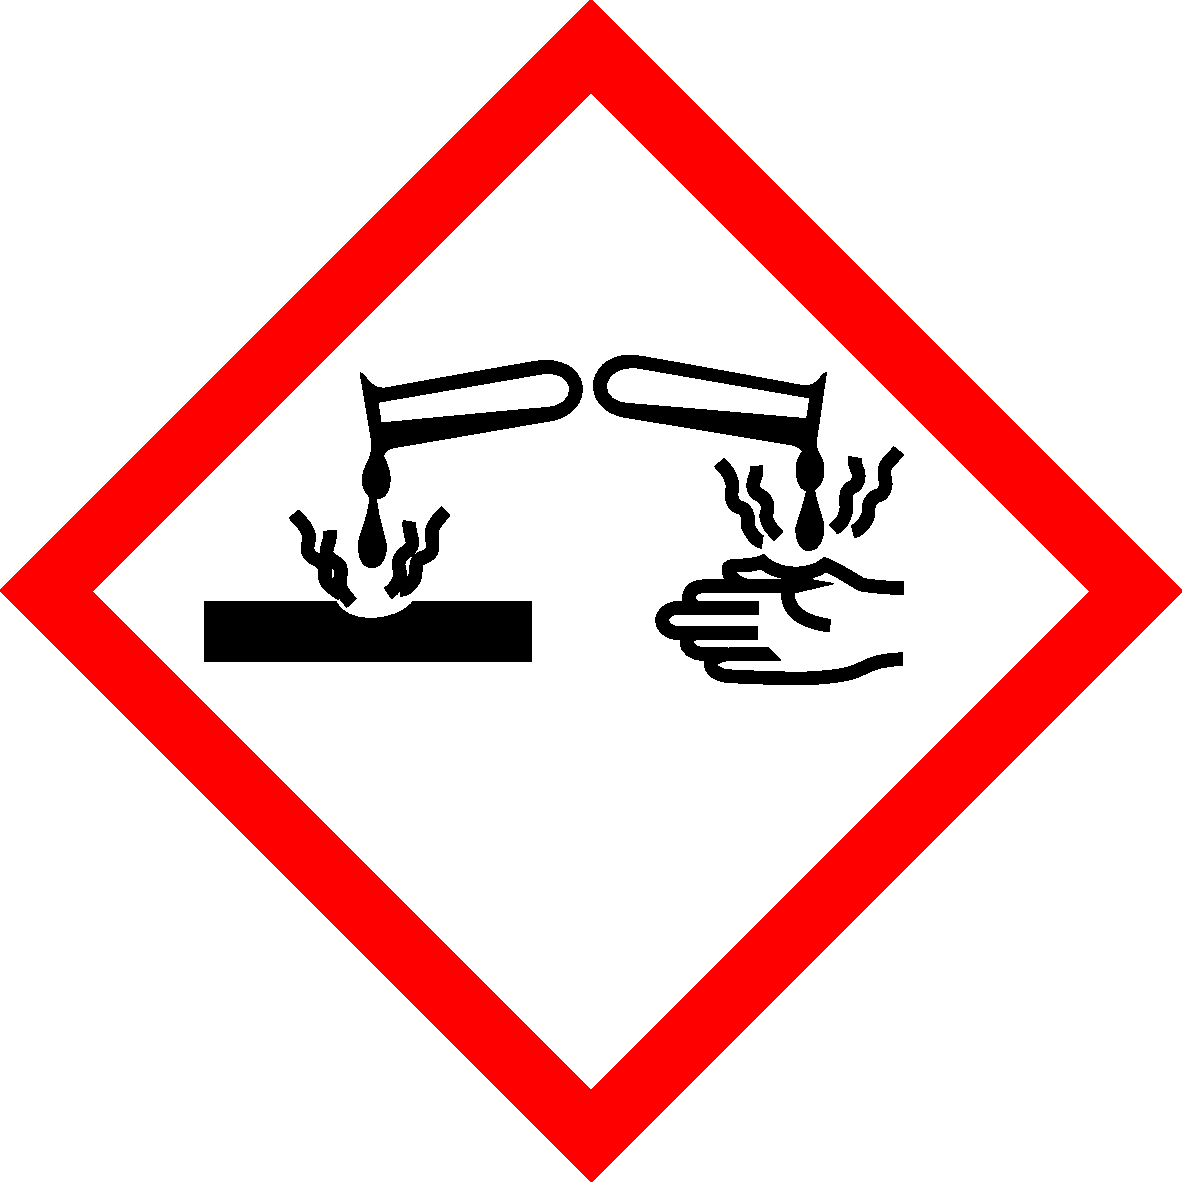
\includegraphics[width=1cm]{pictos/corro.pdf}
\includegraphics[width=1cm]{pictos/envi.pdf} & H318 Provoque de graves lésions des yeux ; H373 Risque présumé d'effets graves pour les organes (Cerveau) à la suite d'expositions répétées ou d'une exposition prolongée en cas d'inhalation ; H411 Toxique pour les organismes aquatiques, entraîne des effets néfastes à long terme. \\
\hline
Carbonate de sodium \ce{Na2CO3} & $105.99 ~ \si{\gram\per\mole}$ & 
\includegraphics[width=1cm]{pictos/exclam.pdf} & H319 Provoque une sévère irritation des yeux.\\
\hline
\end{tabular}
\end{center}

\newpage

\section{Analyse thermique : exemple de l'analyse thermogravimétrique}
\label{sec:TGA}
L'analyse thermique englobe une série de techniques visant à examiner l'évolution d'une diversité de propriétés physiques d'un matériau en réponse à des variations de température, de durée et de composition atmosphérique. Parmi les paramètres observables figurent le flux thermique et la masse. La panoplie de méthodes disponibles comprend au moins une dizaine d'approches distinctes. Ces techniques revêtent une importance significative dans le domaine industriel, notamment pour les applications de contrôle qualité.

L'analyse thermogravimétrique, notée ATG, est une méthode qui permet de suivre la masse d'un échantillon en fonction de la température et de quantifier la perte ou la prise de masse de l'échantillon. Elle sera étudiée en détails au semestre prochain dans le module \emph{MAT4.13 : Alliages} et utilisée en \emph{synthèse inorganique 4.10}.

\subsection{Considérations générales}

L'ATG est une technique permettant d'étudier principalement la \textbf{stabilité}, la \textbf{cinétique} et la \textbf{décomposition} thermique d'un échantillon solide.

\begin{figure}[H]
\begin{minipage}{0.73\textwidth}\centering
\subfloat[\label{fig:Ann02}]{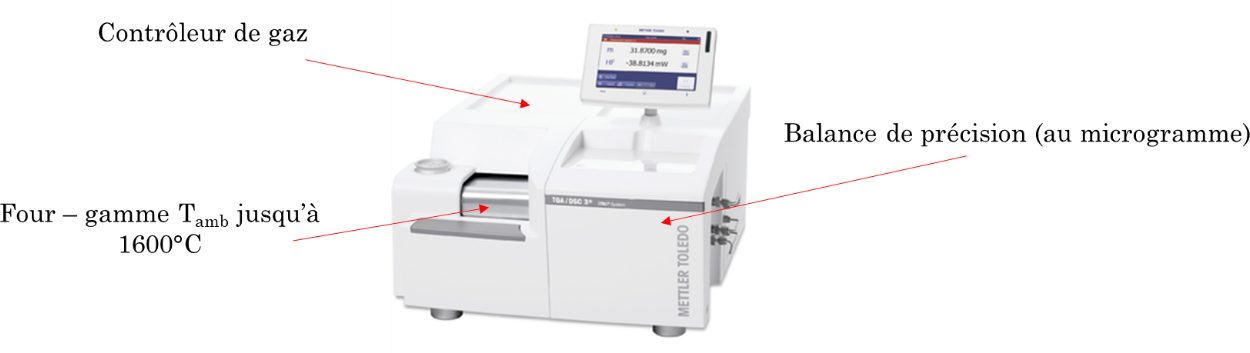
\includegraphics[height=4cm]{figures/Ann02}}\hspace{1cm}\subfloat[\label{fig:Ann03}]{
\includegraphics[width=3cm]{figures/Ann03}}
\end{minipage}\hfill\begin{minipage}{0.23\textwidth}
\caption{\ref{fig:Ann02} Appareil d'ATG/DSC utilisé à l'IUT d'Orsay ; \ref{fig:Ann03} Porte échantillon contenu dans le four.}
\end{minipage}
\end{figure}

Vous placez votre échantillon sur l'emplacement prévu à cet effet (cf. \ref{fig:Ann02}) contenu dans un creuset. \`{A} l'IUT, le creuset est soit : 
\begin{enumerate}
\item en aluminium (bonne conductivité thermique, risque de réaction avec l'échantillon, température tolérable maximale de \SI{600}{\celsius}) 
\item en alumine (faible conductivité thermique, inerte chimiquement, toute la gamme de température). 
\end{enumerate}

L'une des expériences possibles, et couramment réalisée à l'IUT, consiste à faire changer la température du four selon une séquence prédéfini par l'utilisateur. La séquence la plus simple consiste à réaliser une rampe unique en température, comme illustré ci-dessous : 

\begin{center}
\begin{minipage}{0.48\textwidth}

\includegraphics[width=\textwidth]{figures/Ann04}
\end{minipage}\begin{minipage}{0.48\textwidth}
\captionof{figure}{Séquence simple, constituée d'une seule étape, avec rampe de température.}
\label{fig:04}
\end{minipage}
\end{center}

Le porte échantillon est lié à une balance de précision qui analyse la variation de masse de l'échantillon à chaque instant.

Dans ce type d'expériences, vous pouvez contrôler les paramètres expérimentaux suivants :
\begin{enumerate}
\item la nature chimique et la contenance des creusets ;
\item la masse initiale de l'échantillon (généralement entre 0-\SI{30}{\milli\gram}) ;
\item température initiale en \si{\celsius};
\item température finale en \si{\celsius} ;
\item gradient ou rampe de température en \si{\celsius\per\minute} ;
\item la nature chimique de l'atmosphère contrôlées (\emph{par ex.} \ce{O2}, \ce{N2}, \ce{H2}, \ce{Ar}$\ldots$) et le débit de gaz ;
\item le pas de temps d’échantillonnage de la masse.
\end{enumerate}%Nature du creuset ?

\subsection{Exemple d'expérience de décomposition : étude d'un mélange}

Par exemple, vous disposez d'un mélange \textbf{équimassique} d'aluminium et de manganèse, précipités en condition basique sous la forme d'hydroxyde d'aluminium \ce{Al(OH)3} et d'hydroxyde de magnesium \ce{Mg(OH)2}. Les précipités n'ont été que partiellement séchés. \`{A} partir de ce mélange, l'expérimentateur obtient le \textbf{thermogramme} (c.-à-d. la masse de l'échantillon par rapport à la masse initiale en fonction de la température ou du temps d'acquisition) suivant :

\begin{center}
\begin{minipage}{0.48\textwidth}

\includegraphics[width=\textwidth]{figures/Ann01}
\end{minipage}\hfill\begin{minipage}{0.48\textwidth}
\captionof{figure}{Thermogramme réalisé sous atmosphère contrôlé d'un mélange d'hydroxydes d'aluminium et de magnésium.}
[Creuset aluminium de contenance \SI{70}{\micro\liter} ; échantillon \SI{20}{\milli\gram} ; atmosphère \ce{N2 (g)} à un débit de \SI{200}{\milli\liter\per\minute} entre 35 et \SI{600}{\celsius} et atmosphère \ce{O2 (g)} à un débit de \SI{200}{\milli\liter\per\minute} entre 600 et \SI{850}{\celsius}, rampe : \SI{30}{\celsius\per\minute}]
\end{minipage}
\end{center}

Le thermogramme montre une légère perte de masse initiale entre 35 et \SI{200}{\celsius} associée aux traces d'eau encore présentes dans l'échantillon (c.-à-d. une évaporation des résidus d'eau).

Ensuite, le thermogramme donne deux décompositions successives associées qui correspondent, d'après la littérature, à deux déshydratations : 
\begin{enumerate}
\item une perte de masse de \SI{15.05}{\percent} dont le point d'inflection est situé à \SI{300}{\celsius} correspondant à la déshydratation de l'hydroxyde d'aluminium : 
\begin{align}
\ce{2 Al(OH)3 (s) -> Al2O3 (s) + 3 H2O (g)} \label{eq:Al2O3}
\end{align}
\item une perte de masse de \SI{17.7}{\percent} dont le point d'inflection est situé à \SI{415}{\celsius} correspondant à la déshydratation de l'hydroxyde de magnésium : 
\begin{align}
\ce{2 Mg(OH)2 (s) -> MgO (s) + H2O (g)} \label{eq:MgO}
\end{align}
\end{enumerate}

Une perte ou gain de masse en ATG doit être décrit au minimum par : la position du point d'inflexion et la perte relative de masse de l'échantillon. Si vous jouez sur la rampe de température, il peut être important de spécifier l'amplitude en température de la variation de masse.

Pour interpréter les phénomènes de décompositions, il est important de comparer la perte de masse \textbf{expérimentale} à la perte de masse \textbf{théorique} attendue pour une \textbf{réaction totale}. Par exemple, pour \ce{Al2O3}, on a avec l'équation de réaction \ref{eq:Al2O3} :
\begin{align*}
n_0 ( \ce{Al(OH)3} ) = \frac{3}{2} n_\infty ( \ce{H2O} )
\end{align*}
où $n_0 ( \ce{Al(OH)3} )$ (resp. $n_\infty ( \ce{H2O} )$) désigne la quantité de matière initiale (resp. finale) de \ce{Al(OH)3} (resp. \ce{H2O} gazeux)

On peut alors calculer facilement la perte de masse de l'hydroxyde d'aluminium : 
\begin{align*}
\%_{perdu} = \frac{\text{masse perdue}}{\text{masse initiale en \ce{Al2O3}}} \\
= \frac{m_\infty ( \ce{H2O} )}{m_0 ( \ce{Al2O3} ) )} = \frac{3 M( \ce{H2O} )}{2 M( \ce{Al(OH)3} )}
\end{align*}
où $m_0 ( \ce{X} )$ (resp. $m_\infty ( \ce{X} )$) est la masse initiale (resp. finale) du composé X.

On trouve une perte de masse \SI{34.6}{\percent}, soit \SI{17.3}{\percent} de la masse totale de l'échantillon (car $m_0 ( \ce{Al(OH)3} ) = m_0 (\ce{Mn(OH)2})$). Vous constatez un écart de perte de masse de -\SI{2.25}{\percent}, qui indique que l'on a perdu \textbf{moins d'eau} qu'attendu ! Pourquoi ? Les expérimentateurs ont avancé l'hypothèse que l'échantillon initial contient une fraction de \ce{AlO(OH)} qui conduit à la perte de moins d'eau.

\textbf{Vérifiez que vous avez bien compris comment prédire une perte de masse en traitant le cas de Mg.} Vous devez trouver une perte de masse totale du mélange de \SI{15.5}{\percent} de sa masse initiale.


%\subsection{Analyse thermogravimétrique}
%\label{sec:TGA}

%L'analyse thermogravimétrique est une méthode qui permet de suivre la masse d'un échantillon en fonction de la température et de quantifier la perte ou la prise de masse de l'échantillon : elle sera étudiée au S4. 


%\subsection{Calorimétrie différentielle à balayage}
%\label{sec:DSC}

%Nous allons utiliser la calorimétrie différentielle à balayage pendant cette séance. C'est une technique de choix pour étudier des transitions de phase ou des phénomènes de cristallisation.  

\newpage

\section{Diffractogrammes et tables de diffraction sur poudre}
\label{sec:diffracto}
Les simulations sont réalisées via VESTA en considérant une seule longueur d'onde, de valeur $\lambda = 1.542 ~ \si{\angstrom}$

\subsection{\ce{MnSO4.H2O} : $C12/c1$ - 15}

\begin{center}
\begin{adjustbox}{max height=0.70\textwidth}
\begin{tabular}{cccccc}
\toprule
$h$ & $k$ & $l$ & $d$ & $2 \theta$ & I \\
 & & & \si{\angstrom} &  \si{\degree} &  \\  
\midrule
 1 & 1 & -1 &  4.915029 &  18.05005 &  34.00679 \\
 1 & 1 &  0 &  4.856716 &  18.26861 &  25.99867 \\
 0 & 2 &  0 &  3.833500 &  23.20512 &   7.77983 \\
 1 & 1 & -2 &  3.505482 &  25.41116 & 100.00000 \\
 0 & 0 &  2 &  3.492897 &  25.50426 &   0.55882 \\
 1 & 1 &  1 &  3.442601 &  25.88329 &  22.00735 \\
 0 & 2 &  1 &  3.360737 &  26.52515 &  35.27318 \\
 2 & 0 & -2 &  3.202022 &  27.86580 &   0.49828 \\
 2 & 0 &  0 &  3.138315 &  28.44325 &  48.79656 \\
 2 & 2 & -1 &  2.607416 &  34.39844 &  16.00856 \\
 0 & 2 &  2 &  2.581885 &  34.74935 &  42.02455 \\
 1 & 1 & -3 &  2.481898 &  36.19674 &   0.65508 \\
 2 & 2 & -2 &  2.457514 &  36.56852 &   2.24339 \\
 1 & 1 &  2 &  2.444539 &  36.76956 &   4.78512 \\
 2 & 2 &  0 &  2.428358 &  37.02342 &   0.82234 \\
 1 & 3 & -1 &  2.373637 &  37.90910 &   1.01458 \\
 1 & 3 &  0 &  2.366978 &  38.01983 &  11.18871 \\
 3 & 1 & -2 &  2.244623 &  40.17900 &  17.48451 \\
 3 & 1 & -1 &  2.227849 &  40.49471 &   0.56549 \\
 1 & 3 & -2 &  2.144365 &  42.14475 &   8.24431 \\
 1 & 3 &  1 &  2.129726 &  42.44841 &   2.90050 \\
 2 & 2 & -3 &  2.107933 &  42.90886 &  10.20852 \\
 2 & 2 &  1 &  2.071438 &  43.70336 &   2.05050 \\
 3 & 1 & -3 &  2.056460 &  44.03826 &   0.15590 \\
 3 & 1 &  0 &  2.018408 &  44.91330 &  12.19842 \\
 0 & 2 &  3 &  1.990199 &  45.58543 &   2.28708 \\
 2 & 0 & -4 &  1.970800 &  46.05983 &   6.40624 \\
 2 & 0 &  2 &  1.926418 &  47.18445 &   0.05235 \\
 0 & 4 &  0 &  1.916750 &  47.43700 &   3.42476 \\
 1 & 1 & -4 &  1.875509 &  48.54645 &   7.08309 \\
 1 & 1 &  3 &  1.852837 &  49.17956 &   0.69394 \\
 0 & 4 &  1 &  1.848434 &  49.30450 &   0.06522 \\
 1 & 3 & -3 &  1.830518 &  49.81977 &   0.96784 \\
 1 & 3 &  2 &  1.815374 &  50.26410 &   0.84157 \\
 3 & 1 & -4 &  1.780538 &  51.31813 &   0.46862 \\
 4 & 0 & -2 &  1.778451 &  51.38274 &   2.26945 \\
 2 & 2 & -4 &  1.752741 &  52.19276 &   6.00821 \\
 0 & 0 &  4 &  1.746448 &  52.39509 &   2.29910 \\
 3 & 1 &  1 &  1.739654 &  52.61537 &   0.67592 \\
 3 & 3 & -2 &  1.728840 &  52.97002 &   1.45401 \\
 2 & 2 &  2 &  1.721301 &  53.22025 &  16.37358 \\
 3 & 3 & -1 &  1.721141 &  53.22557 &   0.20380 \\
 2 & 4 & -1 &  1.687347 &  54.37841 &   0.50717 \\
 0 & 4 &  2 &  1.680368 &  54.62301 &   7.73661 \\
 2 & 4 & -2 &  1.644610 &  55.91340 &   9.80152 \\
 3 & 3 & -3 &  1.638343 &  56.14617 &   2.41437 \\
 2 & 4 &  0 &  1.635785 &  56.24176 &   0.40524 \\
 3 & 3 &  0 &  1.618905 &  56.88124 &   8.87728 \\
 4 & 2 & -2 &  1.613294 &  57.09723 &   3.54419 \\
 4 & 0 & -4 &  1.601011 &  57.57608 &   6.87792 \\
 0 & 2 &  4 &  1.589291 &  58.04094 &   1.16862 \\
 4 & 2 & -3 &  1.579747 &  58.42536 &   2.03844 \\
 4 & 0 &  0 &  1.569157 &  58.85824 &   2.02960 \\
 4 & 2 & -1 &  1.564210 &  59.06282 &   1.11543 \\
 1 & 3 & -4 &  1.542328 &  59.98591 &   6.61801 \\
 1 & 3 &  3 &  1.529646 &  60.53506 &   0.21605 \\
 2 & 4 & -3 &  1.526415 &  60.67664 &   0.24794 \\
 3 & 1 & -5 &  1.515546 &  61.15824 &   0.17070 \\
 2 & 4 &  1 &  1.512386 &  61.29977 &   1.37305 \\
 1 & 1 & -5 &  1.495338 &  62.07547 &   0.14975 \\
 1 & 5 & -1 &  1.491247 &  62.26473 &   0.08867 \\
 1 & 5 &  0 &  1.489592 &  62.34166 &   2.22516 \\
 3 & 3 & -4 &  1.488201 &  62.40647 &   2.44562 \\
 1 & 1 &  4 &  1.480515 &  62.76712 &   1.32878 \\
 3 & 1 &  2 &  1.480266 &  62.77887 &   3.46019 \\
 0 & 4 &  3 &  1.479884 &  62.79694 &   1.50419 \\
 4 & 2 & -4 &  1.477347 &  62.91709 &   2.19165 \\
 3 & 3 &  1 &  1.464080 &  63.55344 &   0.11731 \\
 2 & 2 & -5 &  1.463408 &  63.58607 &   0.95827 \\
 4 & 2 &  0 &  1.452208 &  64.13467 &   1.41555 \\
 2 & 2 &  3 &  1.438963 &  64.79673 &   1.14092 \\
 1 & 5 & -2 &  1.429068 &  65.30092 &   2.10579 \\
 1 & 5 &  1 &  1.424710 &  65.52565 &   0.02974 \\
 5 & 1 & -3 &  1.395302 &  67.08679 &   0.09048 \\
 5 & 1 & -2 &  1.388561 &  67.45605 &   1.02259 \\
 2 & 4 & -4 &  1.374058 &  68.26543 &   0.04888 \\
 2 & 4 &  2 &  1.358752 &  69.14275 &   2.95271 \\
 5 & 1 & -4 &  1.348856 &  69.72311 &   0.88358 \\
\bottomrule
\end{tabular}
\end{adjustbox}
\end{center}

\subsection{\ce{Li2CO3} : $C12/c1$ - 15}

\begin{center}
\begin{adjustbox}{max height=0.75\textwidth}
\begin{tabular}{cccccc}
\toprule
$h$ & $k$ & $l$ & $d$ & $2 \theta$ & I \\
 & & & \si{\angstrom} &  \si{\degree} &  \\
\midrule
1 & 1 &  0 &  4.158799 &  21.36775 &  71.27506 \\
2 & 0 &  0 &  3.793273 &  23.45468 &  10.65903 \\
1 & 1 & -1 &  3.786529 &  23.49705 &   5.53368 \\
1 & 1 &  1 &  3.027390 &  29.50864 &  22.51390 \\
2 & 0 & -2 &  2.920930 &  30.60998 &  76.04702 \\
0 & 0 &  2 &  2.812295 &  31.82313 & 100.00000 \\
1 & 1 & -2 &  2.627104 &  34.13271 &  28.44713 \\
0 & 2 &  0 &  2.486250 &  36.13119 &  16.88510 \\
3 & 1 & -1 &  2.429809 &  37.00051 &  39.41443 \\
0 & 2 &  1 &  2.273995 &  39.63812 &  14.89757 \\
3 & 1 &  0 &  2.254094 &  40.00294 &   9.31994 \\
3 & 1 & -2 &  2.207768 &  40.87940 &   0.00974 \\
2 & 2 & -1 &  2.115162 &  42.75499 &   2.84337 \\
1 & 1 &  2 &  2.114678 &  42.76525 &   0.56899 \\
2 & 2 &  0 &  2.079400 &  43.52747 &   5.91715 \\
4 & 0 & -2 &  2.012216 &  45.05908 &   1.79229 \\
2 & 0 &  2 &  1.908091 &  47.66558 &   1.25938 \\
4 & 0 &  0 &  1.896637 &  47.97145 &   0.00222 \\
2 & 2 & -2 &  1.893265 &  48.06228 &   1.40163 \\
1 & 1 & -3 &  1.878922 &  48.45259 &   0.14686 \\
3 & 1 &  1 &  1.865109 &  48.83477 &  16.23712 \\
0 & 2 &  2 &  1.862702 &  48.90200 &   4.28205 \\
2 & 2 &  1 &  1.818945 &  50.15857 &   0.05206 \\
3 & 1 & -3 &  1.813208 &  50.32833 &   5.58071 \\
1 & 3 &  0 &  1.619303 &  56.86599 &   4.72982 \\
4 & 2 & -1 &  1.595873 &  57.77888 &   1.83349 \\
1 & 3 & -1 &  1.594560 &  57.83098 &   6.05595 \\
2 & 2 & -3 &  1.585771 &  58.18209 &   2.75041 \\
1 & 1 &  3 &  1.578477 &  58.47692 &   6.00547 \\
5 & 1 & -2 &  1.572467 &  58.72221 &   4.94101 \\
5 & 1 & -1 &  1.565551 &  59.00722 &   3.34440 \\
4 & 2 & -2 &  1.564127 &  59.06627 &   7.43759 \\
2 & 0 & -4 &  1.547100 &  59.78201 &  15.97692 \\
1 & 3 &  1 &  1.520292 &  60.94693 &   0.00003 \\
2 & 2 &  2 &  1.513695 &  61.24104 &   6.29765 \\
4 & 2 &  0 &  1.507957 &  61.49928 &   2.56897 \\
3 & 1 &  2 &  1.505259 &  61.62151 &   4.02945 \\
0 & 2 &  3 &  1.496945 &  62.00148 &   1.18007 \\
5 & 1 & -3 &  1.467953 &  63.36626 &   5.18175 \\
3 & 1 & -4 &  1.464295 &  63.54301 &   0.99698 \\
1 & 3 & -2 &  1.461074 &  63.69955 &   2.92805 \\
4 & 0 & -4 &  1.460465 &  63.72925 &   0.00924 \\
5 & 1 &  0 &  1.451250 &  64.18211 &   0.93293 \\
1 & 1 & -4 &  1.436149 &  64.93926 &   1.57582 \\
4 & 2 & -3 &  1.431396 &  65.18155 &   0.14574 \\
3 & 3 & -1 &  1.424324 &  65.54564 &   6.56794 \\
0 & 0 &  4 &  1.406147 &  66.50185 &   0.81723 \\
6 & 0 & -2 &  1.392472 &  67.24127 &   3.19376 \\
3 & 3 &  0 &  1.386266 &  67.58270 &   0.83478 \\
3 & 3 & -2 &  1.375281 &  68.19636 &   1.73376 \\
1 & 3 &  2 &  1.351883 &  69.54449 &   1.82657 \\
4 & 2 &  1 &  1.348273 &  69.75767 &   0.73761 \\
\bottomrule
\end{tabular}
\end{adjustbox}
\end{center}

\subsection{\ce{MnCO3} : $R\bar{3}c$ - 167}

\begin{center}
\begin{adjustbox}{max height=0.9\textwidth}
\begin{tabular}{cccccc}
\toprule
$h$ & $k$ & $l$ & $d$ & $2 \theta$ & I \\
 & & & \si{\angstrom} &  \si{\degree} &  \\ 
\midrule
 0 & 1 &  2 &  3.653668 &   24.36436 &   28.69036 \\
 1 & 0 &  4 &  2.839959 &   31.50504 &  100.00000 \\
 0 & 0 &  6 &  2.606167 &   34.41544 &    0.46846 \\
 1 & 1 &  0 &  2.386000 &   37.70524 &   19.79455 \\
 1 & 1 &  3 &  2.169499 &   41.63366 &   18.54331 \\
 2 & 0 &  2 &  1.997745 &   45.40362 &   19.77967 \\
 0 & 2 &  4 &  1.826834 &   49.92710 &   10.11122 \\
 0 & 1 &  8 &  1.766957 &   51.74160 &   20.36647 \\
 1 & 1 &  6 &  1.759854 &   51.96602 &   29.09855 \\
 2 & 1 &  1 &  1.554268 &   59.47846 &    2.61624 \\
 1 & 2 &  2 &  1.531734 &   60.44389 &   13.72366 \\
 1 & 0 & 10 &  1.462509 &   63.62974 &    2.37603 \\
 2 & 1 &  4 &  1.450501 &   64.21920 &    9.95994 \\
 2 & 0 &  8 &  1.419979 &   65.77150 &    4.12869 \\
 1 & 1 &  9 &  1.404526 &   66.58862 &    2.91761 \\
 1 & 2 &  5 &  1.397402 &   66.97270 &    1.61409 \\
 3 & 0 &  0 &  1.377558 &   68.06820 &   10.80124 \\
\bottomrule
\end{tabular}
\end{adjustbox}
\end{center}

\subsection{\ce{LiMn2O4} : $Fd\bar{3}m$ - 227}

\begin{center}
\begin{tabular}{cccccc}
\toprule
h & k &  l &  $d$   &  $2 \theta$ & I \\
& & & \si{\angstrom} &  \si{\degree} & I \\
\midrule
1 & 1 & 1 & 4.760253 & 18.64208 &  100.00000 \\
2 & 2 & 0 & 2.915048 & 30.67326 &    0.49398 \\
3 & 1 & 1 & 2.485961 & 36.13553 &   47.74673 \\
2 & 2 & 2 & 2.380126 & 37.80181 &    9.97476 \\
4 & 0 & 0 & 2.061250 & 43.93059 &   56.66713 \\
3 & 3 & 1 & 1.891533 & 48.10907 &   10.59707 \\
4 & 2 & 2 & 1.683004 & 54.53037 &    0.07233 \\
3 & 3 & 3 & 1.586751 & 58.14272 &    1.90201 \\
5 & 1 & 1 & 1.586751 & 58.14272 &   16.86672 \\
4 & 4 & 0 & 1.457524 & 63.87304 &   32.25582 \\
5 & 3 & 1 & 1.393659 & 67.17638 &   12.57605 \\
4 & 4 & 2 & 1.374167 & 68.25928 &    0.02952 \\
\bottomrule
\end{tabular}
\end{center}

\newpage

\section*{Barême}

\begin{minipage}{0.33\textwidth}
Noms-Prénoms du binôme
\end{minipage}\begin{minipage}{0.33\textwidth}
$n^\circ 1$ :
\end{minipage}\begin{minipage}{0.33\textwidth}
$n^\circ 2$ :
\end{minipage}

\begin{questions}
\setcounter{question}{\thefoo}

\titledquestion{Graphes}[1] Qualité des graphes

\titledquestion{Investissement}[2] Variable d'ajustement à la liberté du correcteur en fonction de l'investissement, de la qualité des raisonnements et de la démarche d'investigation du binôme.

\end{questions}

\begin{center}
\gradetable
\end{center}

\end{document}